\documentclass{article}
\usepackage[utf8]{inputenc}
\usepackage{blindtext}
\usepackage{graphicx}
\usepackage{hyperref}
\usepackage[dvipsnames]{xcolor}

\title{Report: Locating Chinese Districts in Any City}
\author{Nan He}
\date{June 2021}

\begin{document}

\maketitle

\section{Introduction}
\subsection{Background}
More and more Chinese works and study overseas in the United States, Canada, and other western countries in recent decades.
Oversea Chinese population in the US grow from $3,347,229$ in 2010 to $4,143,982$ in 2020.\cite{census2010chi, census2020chi}
The growing presence of these new Chinese workers has a significant impact on existing local Chinese communities in major western cities.
Research suggested that the newcomers help to revitalize and transforming old Chinatown. \cite{jia2010chinatown}
They also boost many non-traditional Chinatowns or "Chinese Districts" in various middle-sized cities where the local Chinese population is small.

For international Chinese students like me, the existence of a local Chinatown or "Chinese districts" is important for residential decisions.
The combination of Authentic Chinese and Asian food, Asian supermarkets, and various services in the Chinese language provides a smooth cultural transition for many newcomers. Previous publications support my personal experiences.\cite{zhou2010chinatown} This report focuses on finding the opportunities inside this trend.

\subsection{Business Problem}
One major problem of the Chinese districts in middle-sized western cities is that their distributions are generally obscure, especially for someone who is not Chinese.
When I visited Charlotte and Atlanta the first time, when discussing which areas have good access to Chinese services and goods, every person almost gave different answers.
Some have already lived there for over five years while still have no clear clue whether a "Chinese District" exists and where it is.
Inspired by these experiences, in this report, I will investigate this problem and try to build a tool to find the location of an existing Chinese District for any given city using a data-driven approach.

\subsection{Significance}
This problem has values for two types of users. Firstly, investors can identify potential investments in Chinese venues, especially those who are not local to that city or are not familiar with the Chinese communities. Secondly, for other Chinese students and oversee works who seek to find a comfortable environment in an unfamiliar city.

\section{Data Acquisition and Cleaning}
Two types of data are needed to achieve our goal of finding Chinese districts automatically for a given city or area,

1. Data that tells us what a Chinese district should look like.

2. A target city or area the user wants to investigate.

\subsection{Chinese District Feature Data}

For data 1, I retrieve the location of 5 large Chinatown in the US from \href{https://en.wikipedia.org/wiki/Chinatowns_in_the_United_States}{\textcolor{blue}{this Wikipedia page}}. 
Note that ten are listed on that page, and many of them cluster on the west coast. So I choose only New York, San Francisco, Los Angeles, Chicago, and Huston, to make the data more balanced geographically.
A good starting point to study what defines a Chinese district is from the venues in that area.
Therefore, to extract venue data for those areas, I utilize the Foursquare API, a popular location service provider based in the US.\cite{foursquare}

The latitudes and longitudes of the five selected Chinatowns are:
\begin{figure}[h]
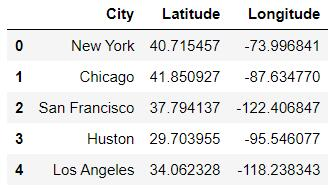
\includegraphics[width=0.5\textwidth]{c1.jpg}
\centering
\end{figure}

Some example resulting venues are:
\begin{figure}[h!]
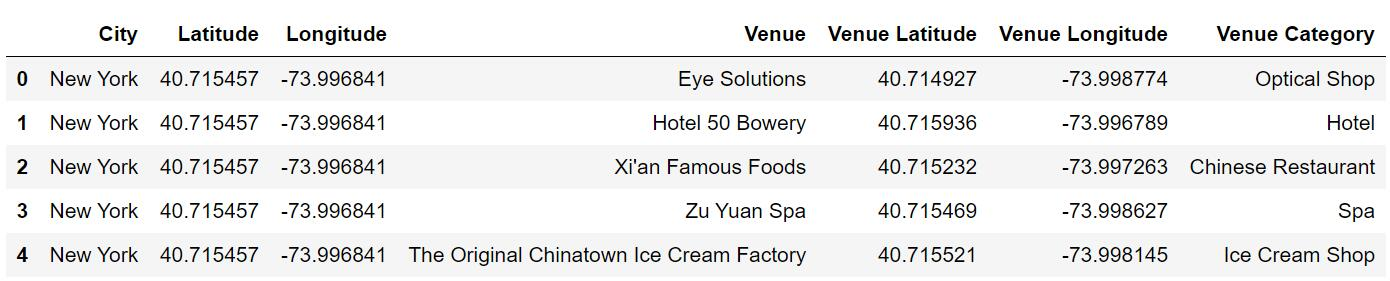
\includegraphics[width=1.0\textwidth]{c2.jpg}
\centering
\end{figure}

In total, 429 venues are selected around these five Chinatowns; those data will tell us what defines a Chinese district.

\newpage

The data will be grouped by the city name and encoded in terms of the venue category. Examples look like:
\begin{figure}[h!]
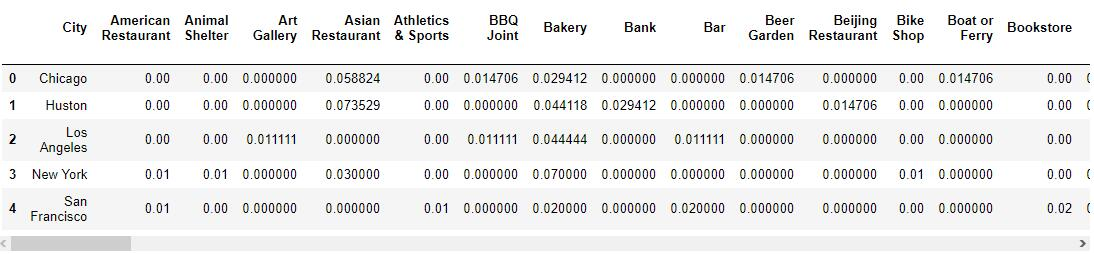
\includegraphics[width=1.0\textwidth]{c2_1.jpg}
\centering
\end{figure}

\subsection{Target City Data}

For data 2, the situation is more complicated.
For each target city, the data sources of neighborhoods vary, making the web-scraping work city-specific.
Here I choose a simple alternative approach.
For each input coordinates user interested, we generate a grid around that latitude and longitude coordinate and analyze the target city based on this grid partition.
Here I take Charlotte, NC, as an example to show how this approach works.

We select two points on google map to select areas include most of the metropolitan area of Charlotte. The grid is constructed by equally partitioning 20$\times$20 sample coordinates within the chosen area.
\begin{figure}[h!]
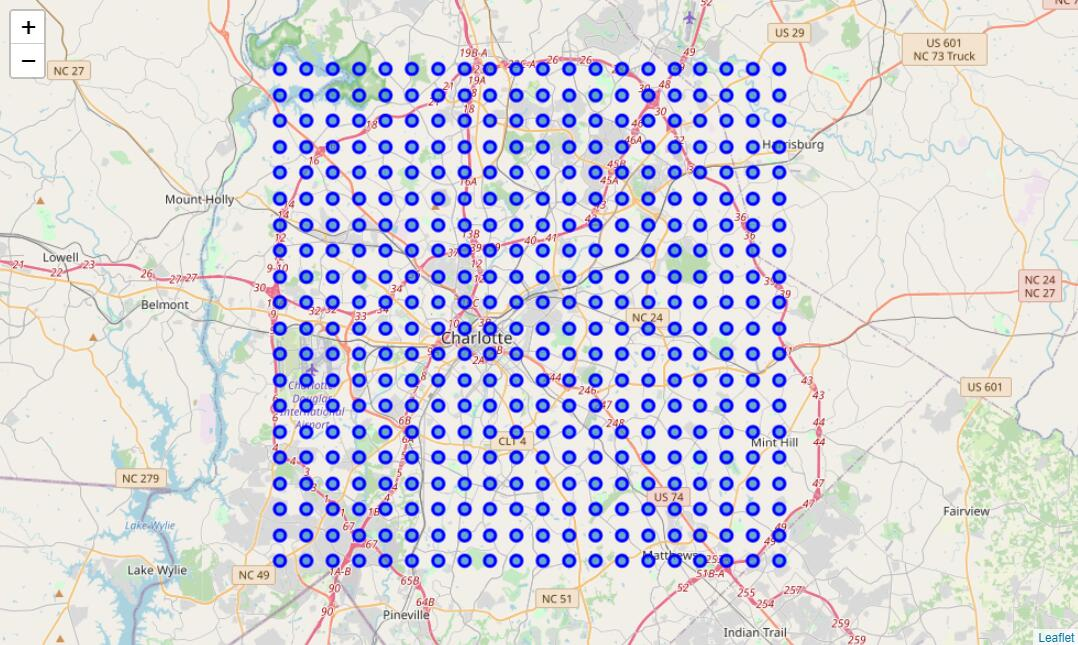
\includegraphics[width=1.0\textwidth]{c3.jpg}
\centering
\end{figure}

Then we loop over those coordinates and find venues within a certain radius of each point. Note that we will make that radius slightly larger than the half-distance of the two diagonal grid points to make sure that no venues are ignored.
In the Charlotte case, the radius is 1500 m.
By taking this approach, there will also have overlapping venues, where the same venues appear in different grid points.
Since the grid points can locate in sparsely populated areas, where the number of venues is tiny, I will ignore them to avoid potential statistical problems. Only grid points with over 15 venues will be appended into the data.

Example venues look like:
\begin{figure}[h!]
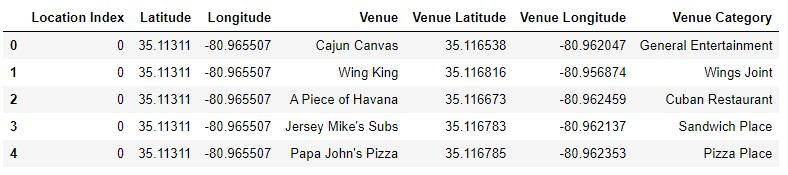
\includegraphics[width=1.0\textwidth]{c4.jpg}
\centering
\end{figure}

In total, 10041 venues are selected. Those data are where we want to get insight from.

Here I show another example to prove the workflow.
Find Atlanta on google map, and select the 
Input point 1 is $33.620260, -84.543165$, point 2 is $34.024354, -84.112095$, and the sample size is 20$\times$20:
\begin{figure}[h!]
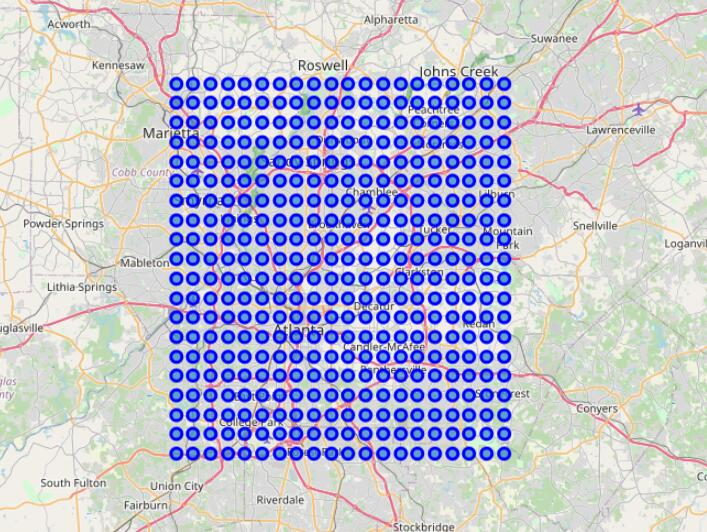
\includegraphics[width=1.0\textwidth]{c5.jpg}
\centering
\end{figure}

\newpage

The data will be grouped by grid point indices and encoded in terms of the venue category. Examples look like:
\begin{figure}[h!]
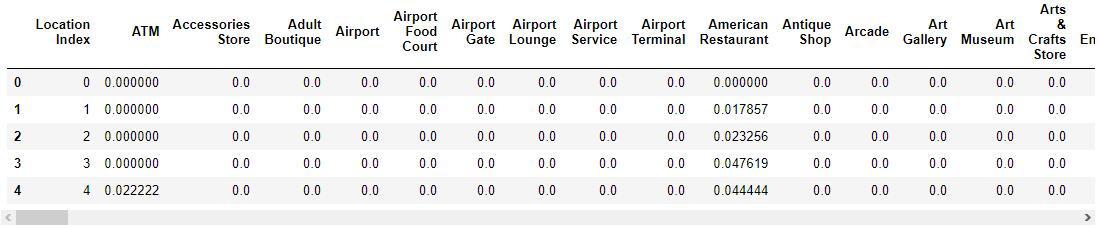
\includegraphics[width=1.0\textwidth]{c6.jpg}
\centering
\end{figure}

Then the data are ready to be analyzed.

\subsection{Usage of the Data}

The most straightforward idea is to use the unsupervised learning techniques only based on the target-city data.
In this case, we do not need data 1.
However, Chinese venues are not typical features for many US cities; it is highly possible that naive unsupervised learning techniques cannot distinguish the Chinese district from other districts.
Therefore, data 1 will play a vital role in screening the venue types and possibly introducing weighted distances during unsupervised learning.

\newpage

\section{Methodology}
\subsection{Naive K-means Clustering}

(Kmeans introduction)

(Naive Kmean approach I take)

\begin{figure}[h!]
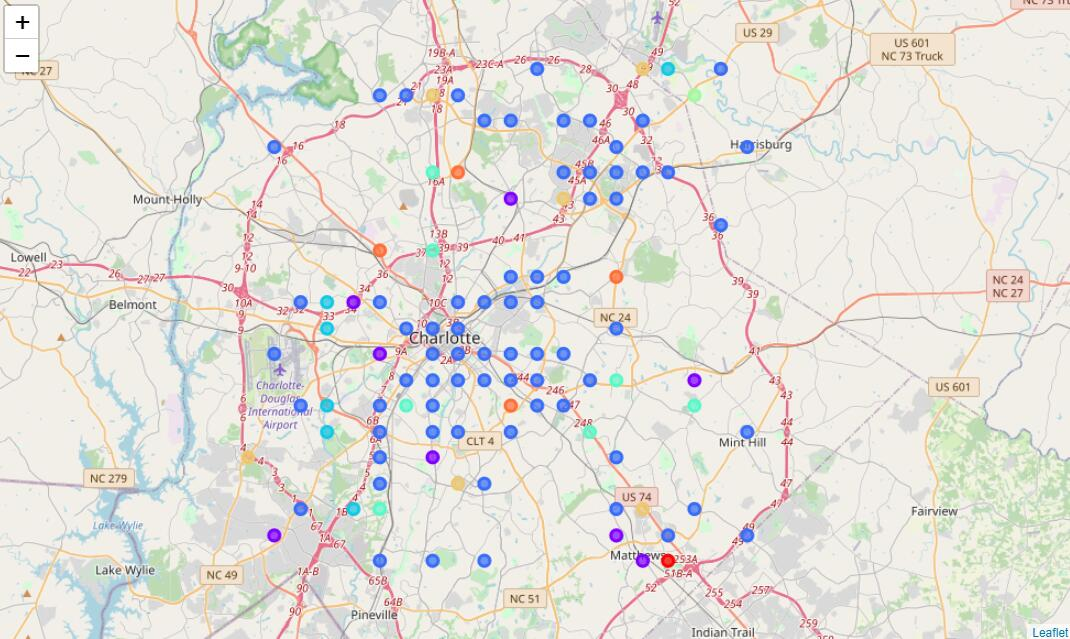
\includegraphics[width=1.0\textwidth]{cn1.jpg}
\centering
\end{figure}

(The problems)

\newpage

\subsection{Feature Analysis}

(Discuss the feature selection)

\begin{figure}[h!]
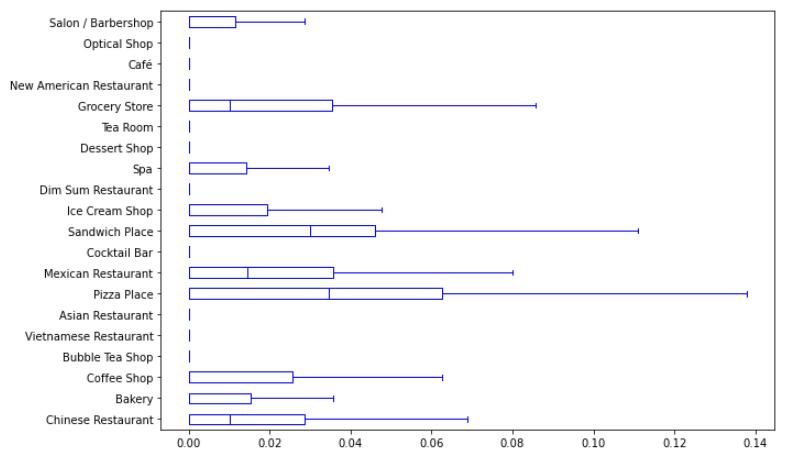
\includegraphics[width=1.0\textwidth]{cn2.jpg}
\centering
\end{figure}

\begin{figure}[h!]
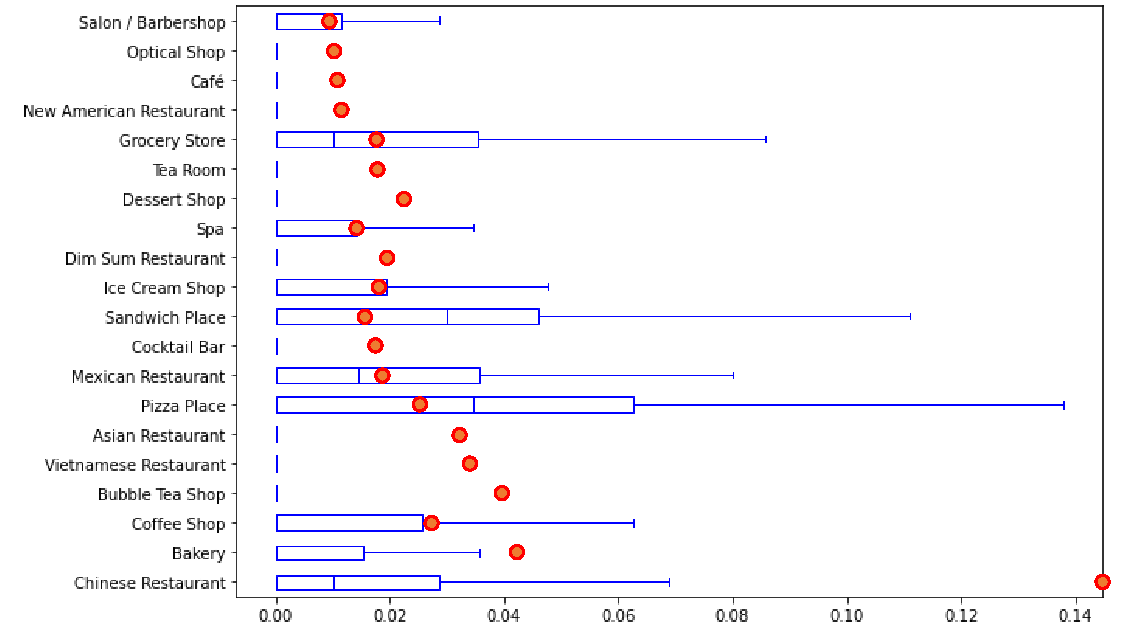
\includegraphics[width=1.0\textwidth]{cn3.pdf}
\centering
\end{figure}

\newpage

\subsection{Weighted Distance K-means}

(Discuss how the distance is weighted)

\newpage

\section{Result and Discussion}

\subsection{Results of Charlotte}

\begin{figure}[h!]
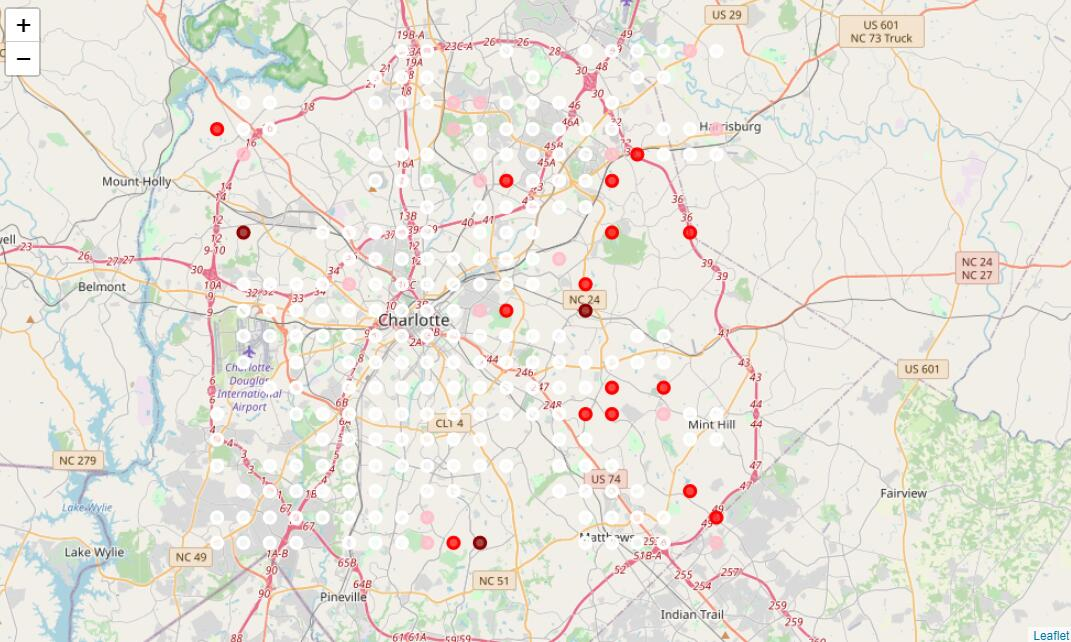
\includegraphics[width=1.0\textwidth]{cn4.jpg}
\centering
\end{figure}

\newpage

\subsection{Results of Atlanta}

\begin{figure}[h!]
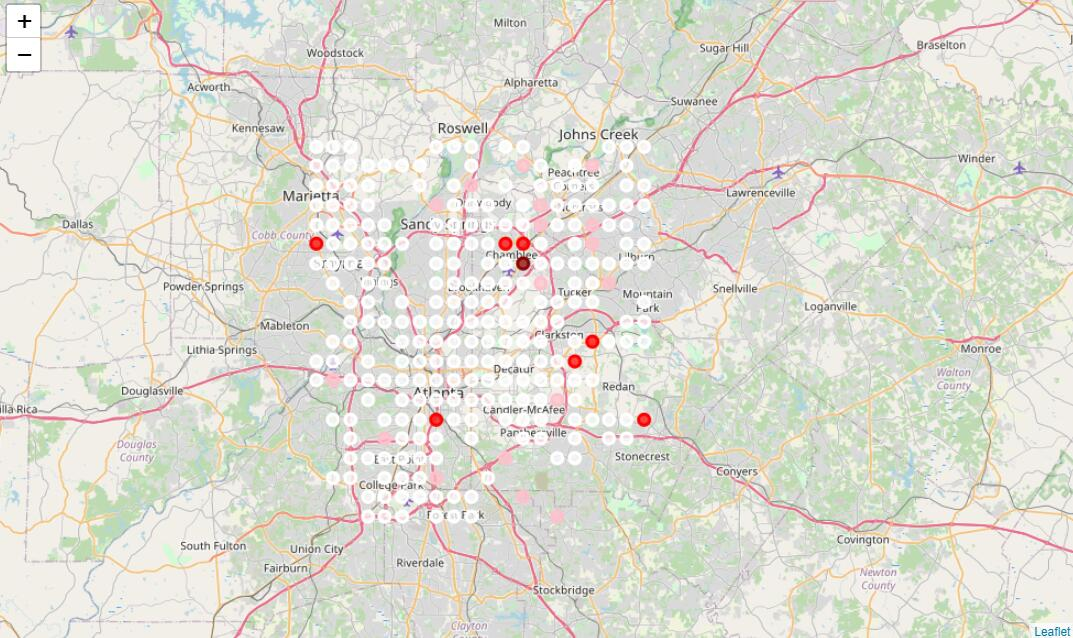
\includegraphics[width=1.0\textwidth]{cn5.jpg}
\centering
\end{figure}

\newpage

\subsection{The Pipeline}

\subsection{Potential Problems}

\section{Conclusion}

\newpage

\bibliographystyle{unsrt}
\bibliography{capstone}

\end{document}
